%note: don't split this document up with include{...}

\part{Sequenzdiagramme}

\section*{Starten des Programms}
\begin{figure}[H]
  \centering
    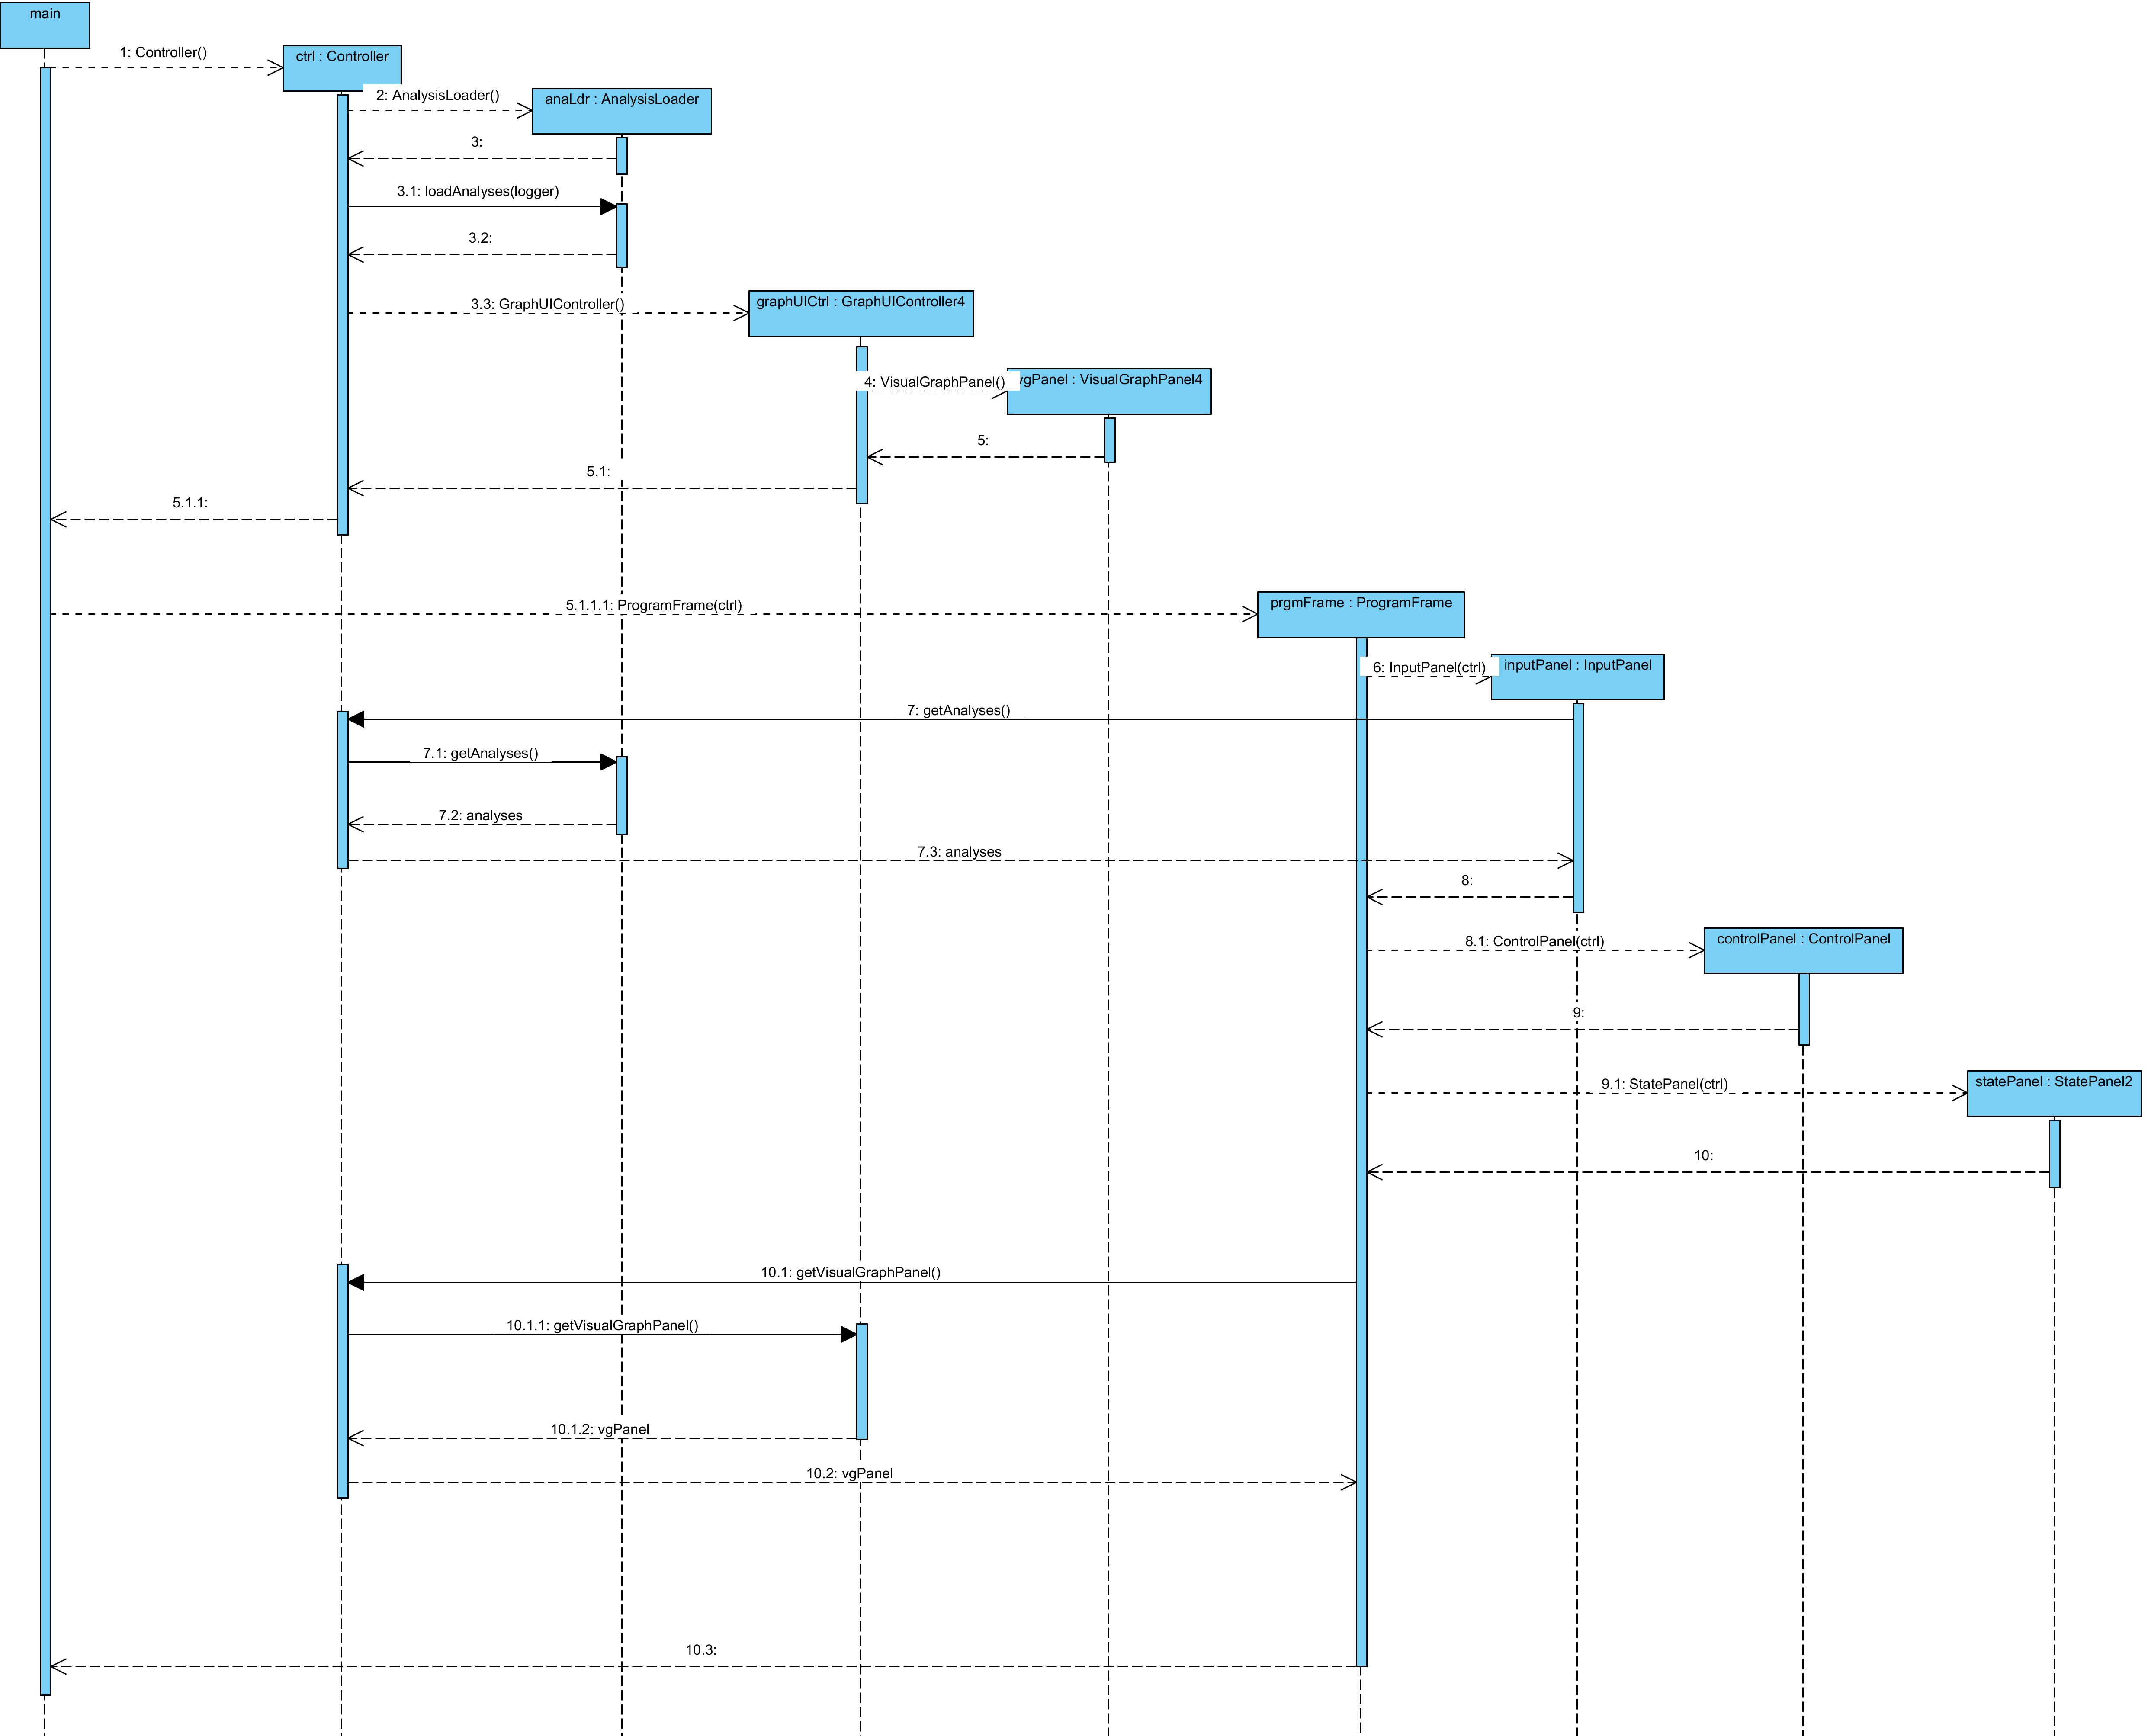
\includegraphics[width=1\textwidth]{Sequenzdiagramme/ProgramStart}
  \caption{Starten des Programms}
  \label{fig:start}
\end{figure}
\FloatBarrier
\clearpage


\section*{Konstruktor der DFAExecution}
\begin{figure}[H]
	\centering
	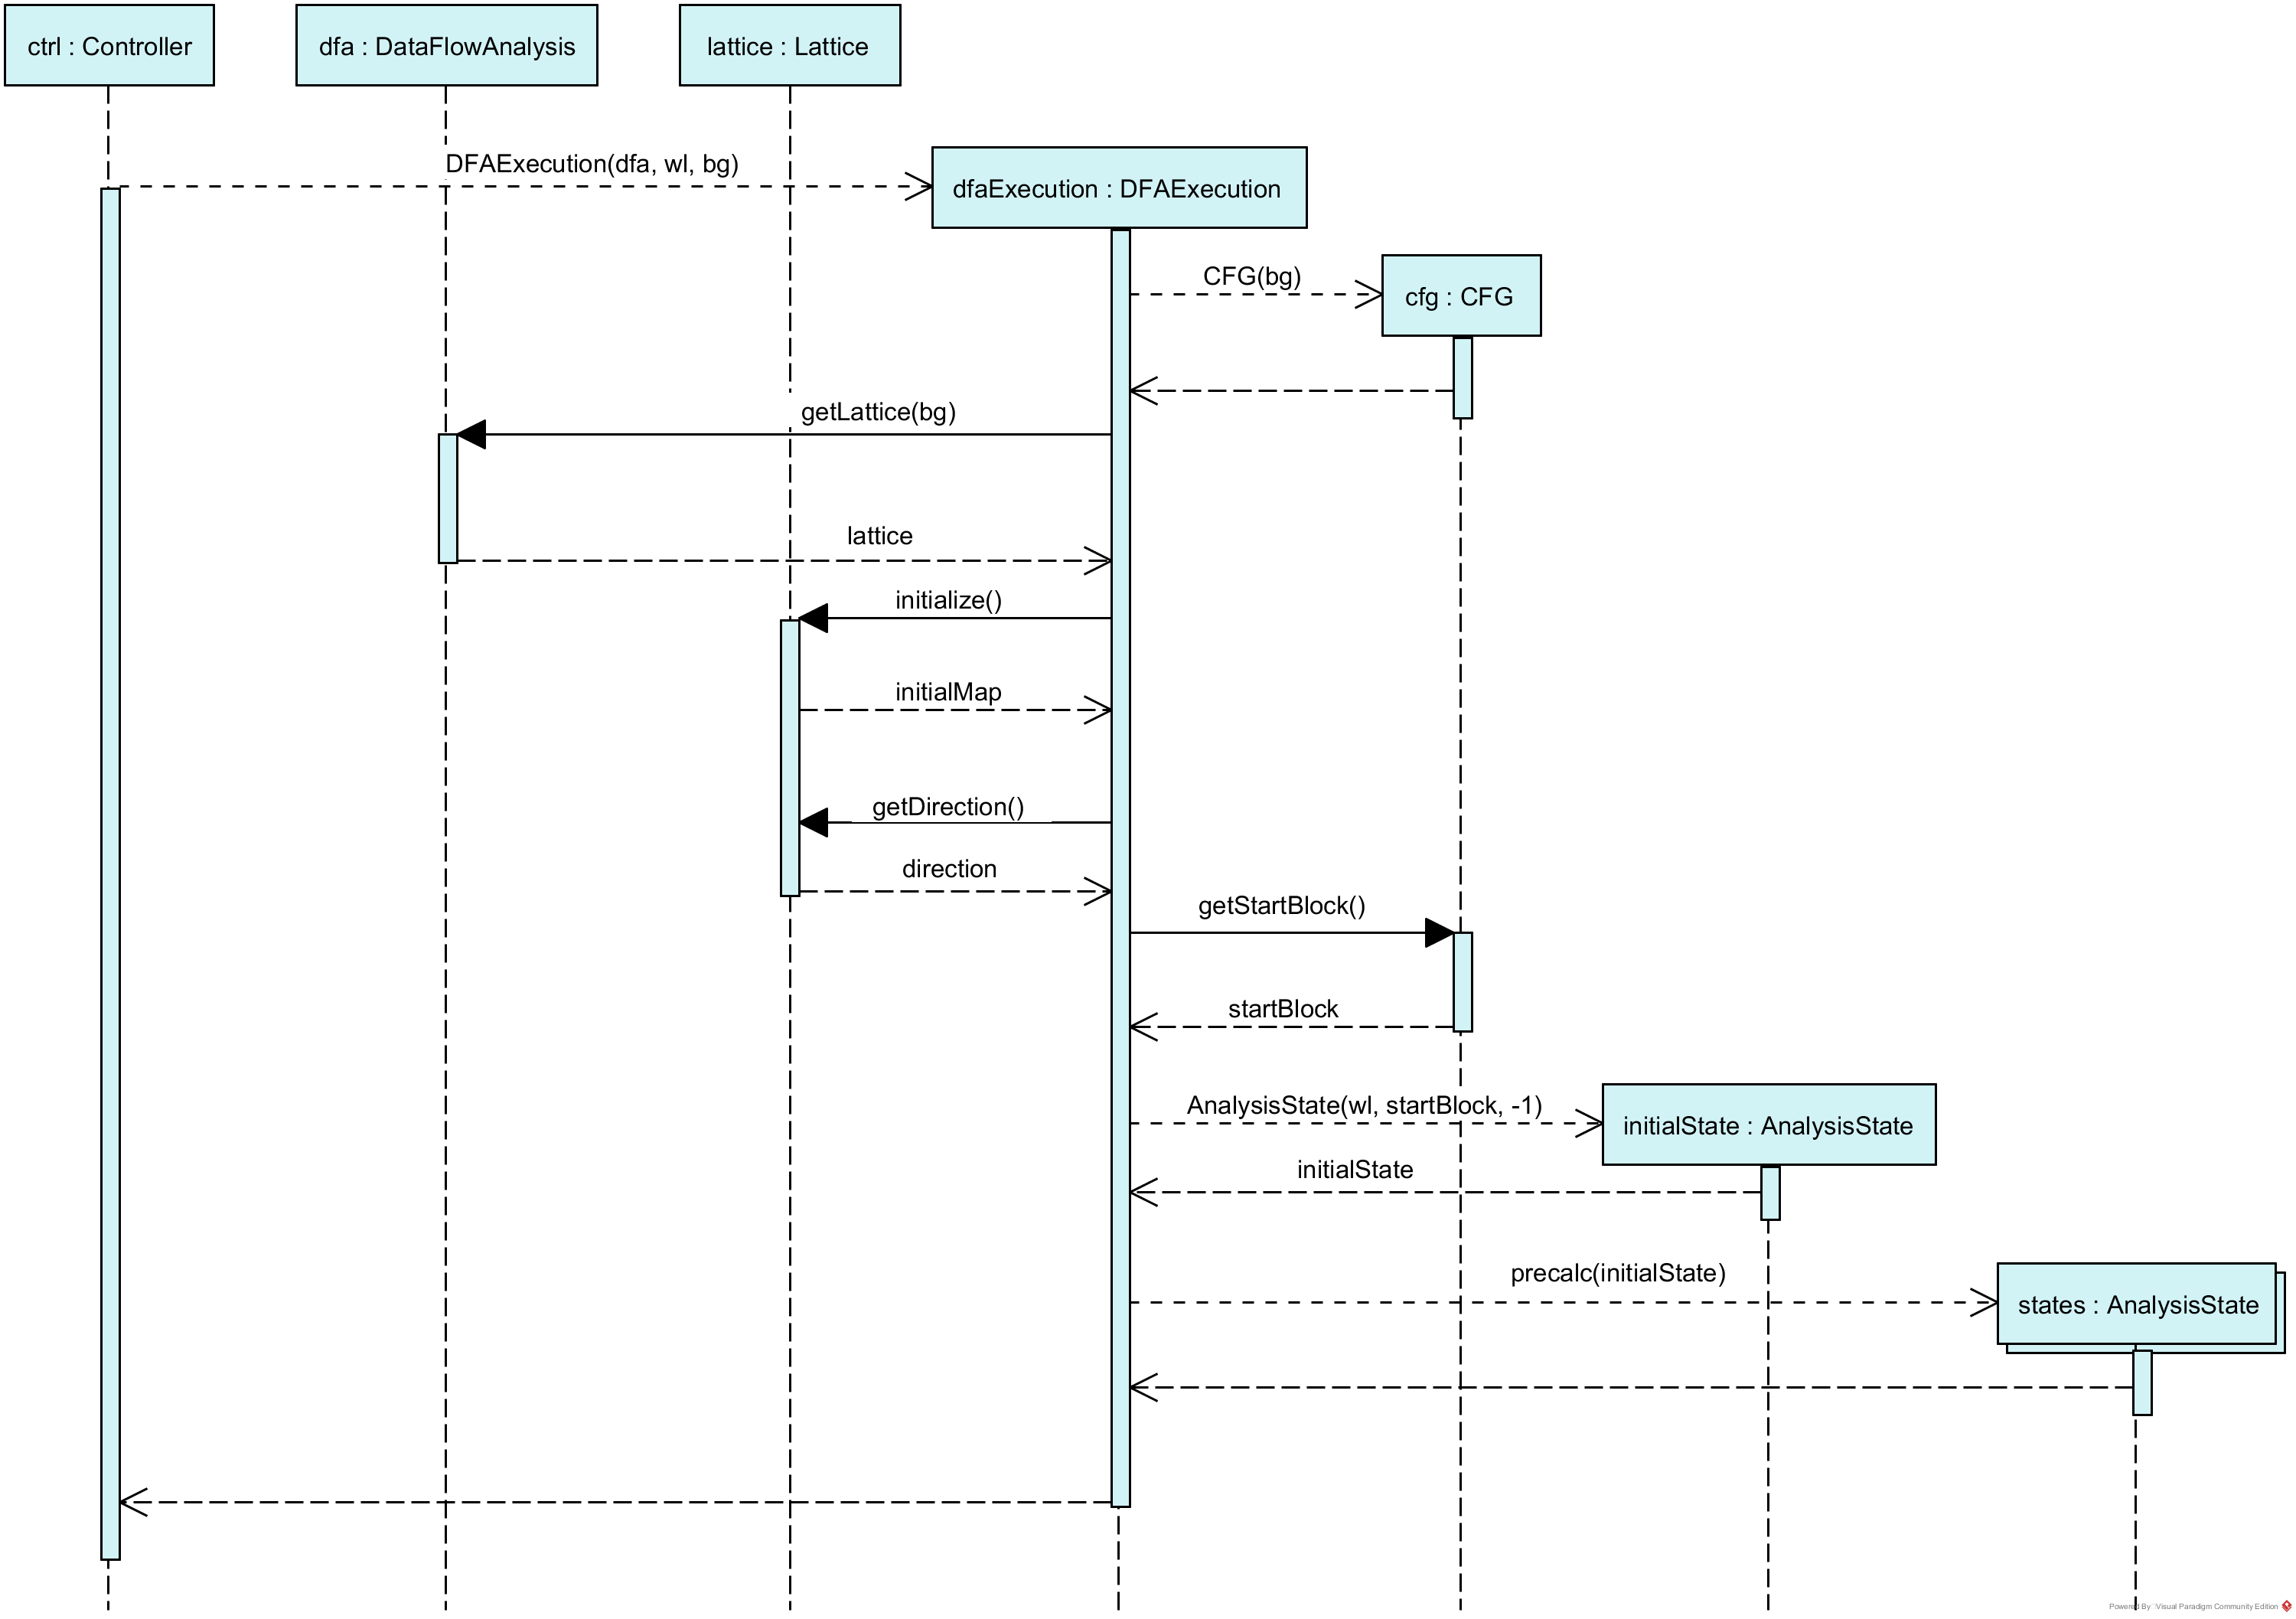
\includegraphics[width=1\textwidth]{Sequenzdiagramme/KonstruktorDFAExecution}
	\caption{Konstruktoraufruf bei der DFAExecution}
	\label{fig:dfactor}
\end{figure}
\FloatBarrier
\clearpage


\section*{Erstellen eines neuen Graphen}
\begin{figure}[H]
  \centering
    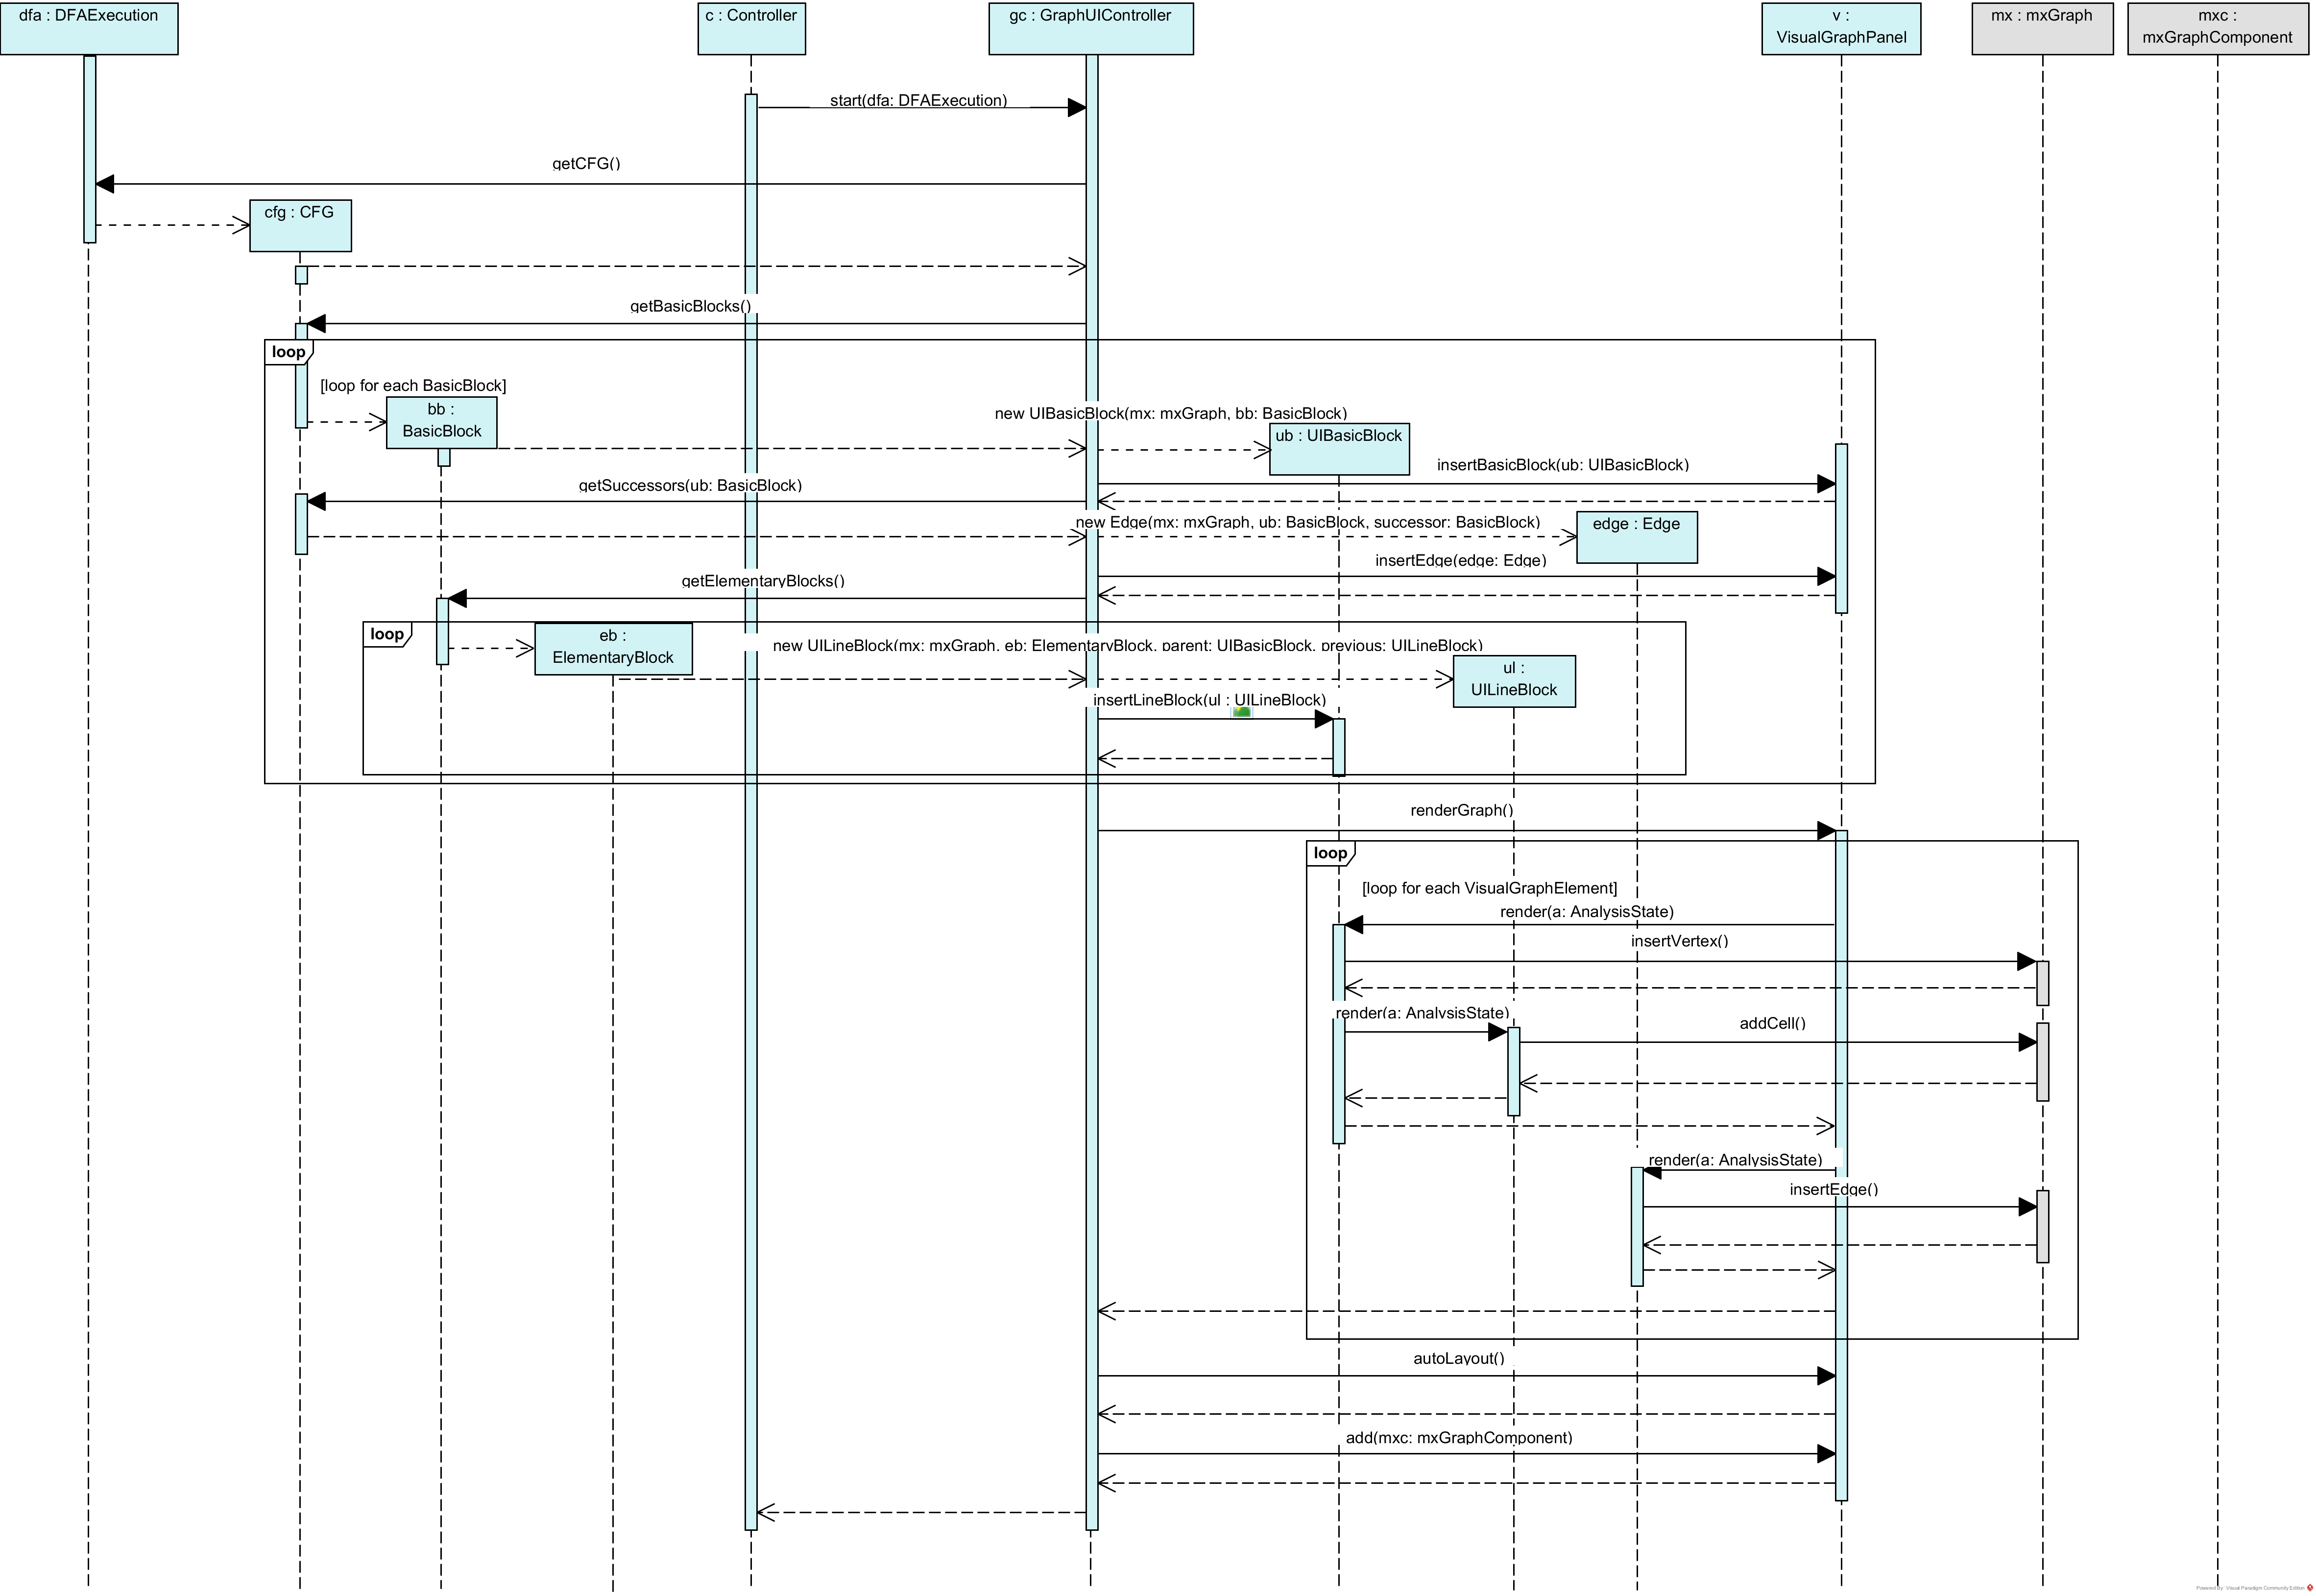
\includegraphics[width=1\textwidth]{Sequenzdiagramme/CreateGraph}
  \caption{Erstellen eines neuen Graphen}
  \label{fig:creategraph}
\end{figure}
\newpage

\section*{Graphen aktualisieren}
\begin{figure}[H]
	\centering
	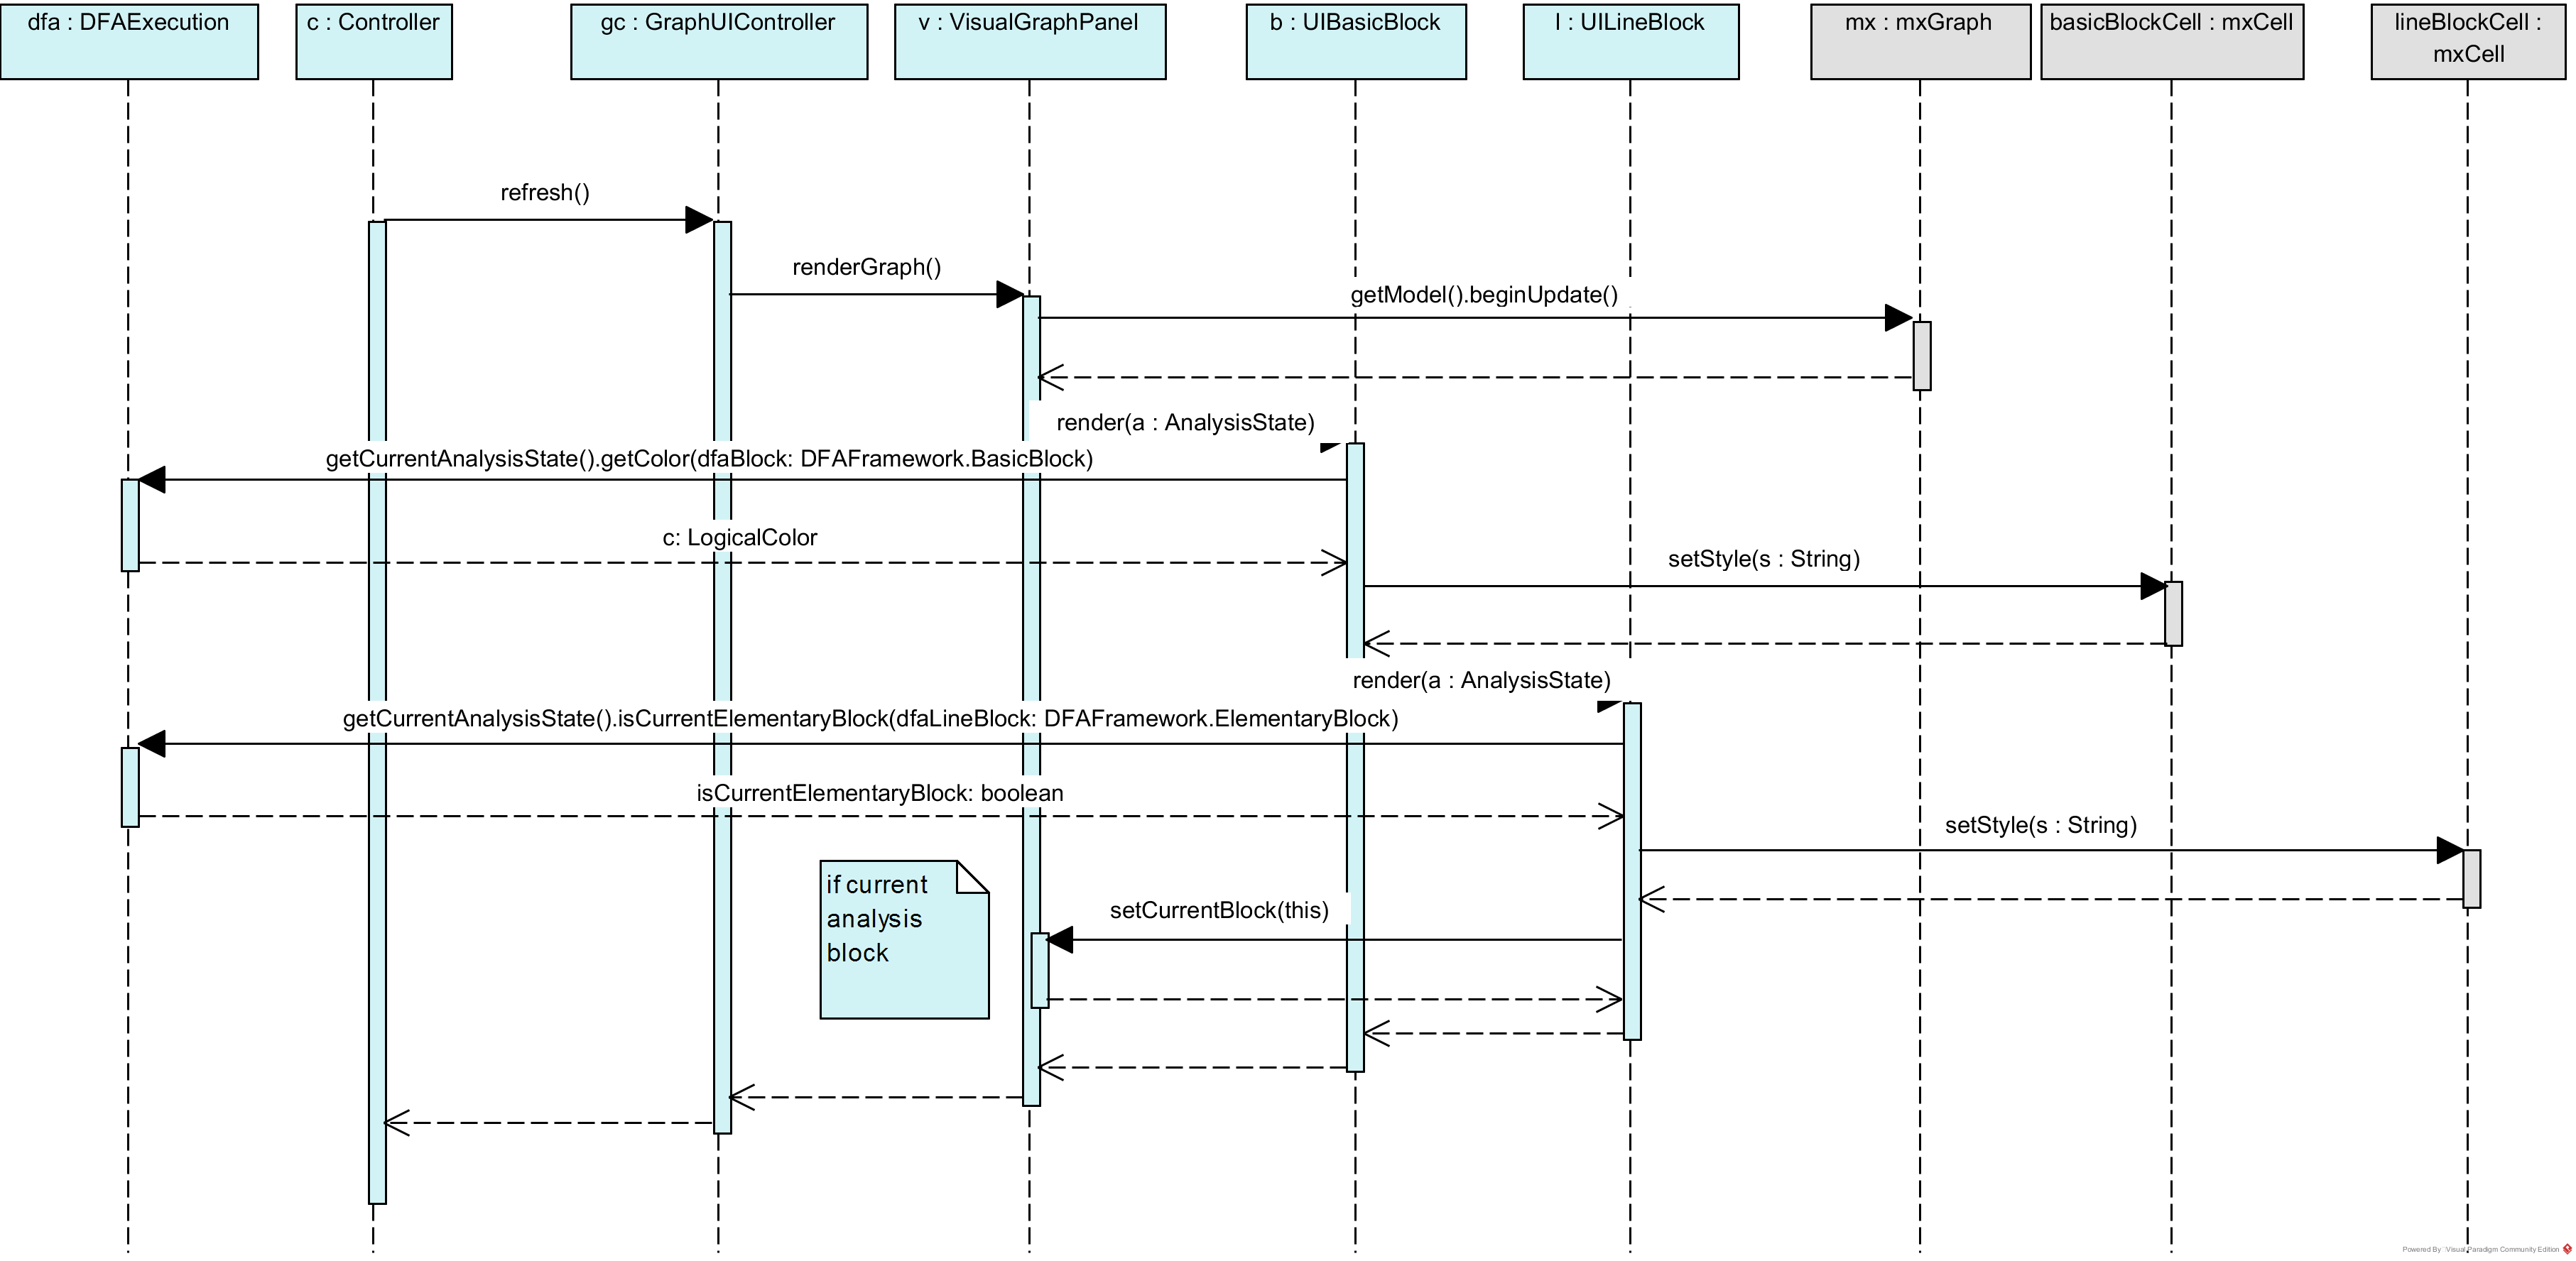
\includegraphics[width=1\textwidth]{Sequenzdiagramme/RefreshGraph}
	\caption{Aktualisieren des Graphen}
	\label{fig:graphrefresh}
\end{figure}
\newpage

\section*{Starten der Analyse}
\begin{figure}[H]
  \centering
    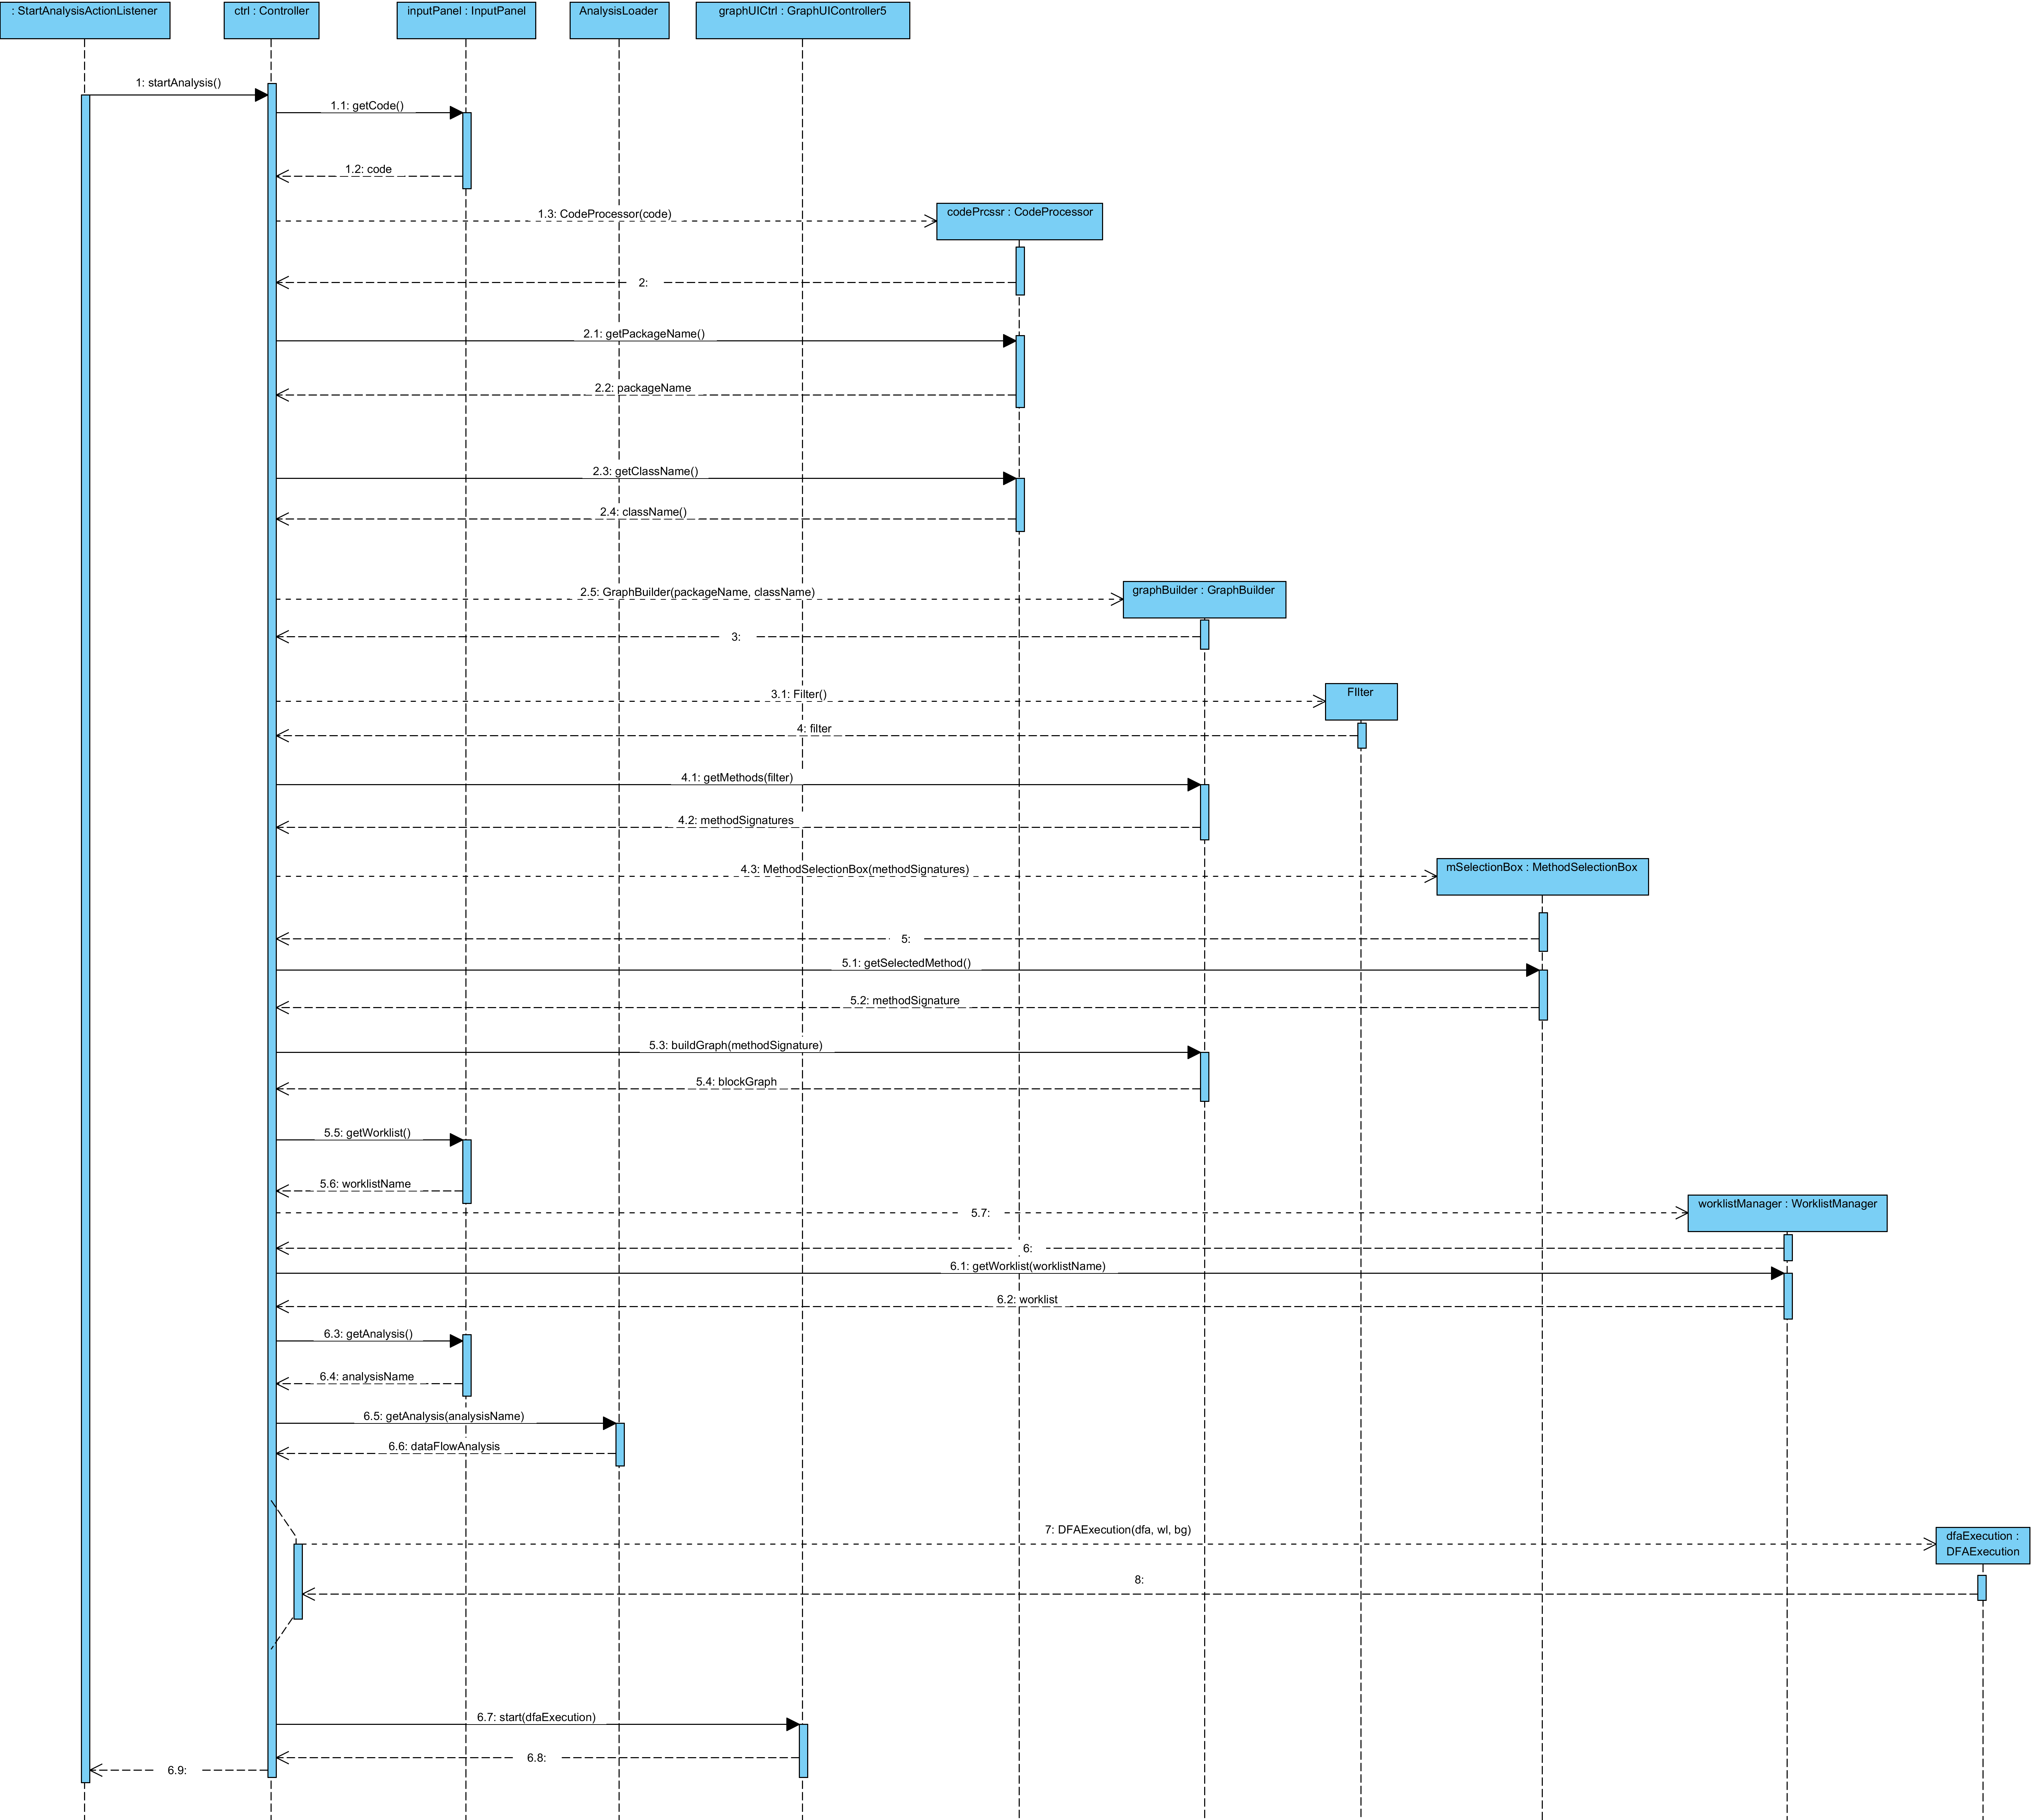
\includegraphics[width=1\textwidth]{Sequenzdiagramme/AnalysisStart}
  \caption{Starten der Analyse}
  \label{fig:anaStart}
\end{figure}
\newpage

\section*{Stoppen der Analyse}
\begin{figure}[H]
  \centering
    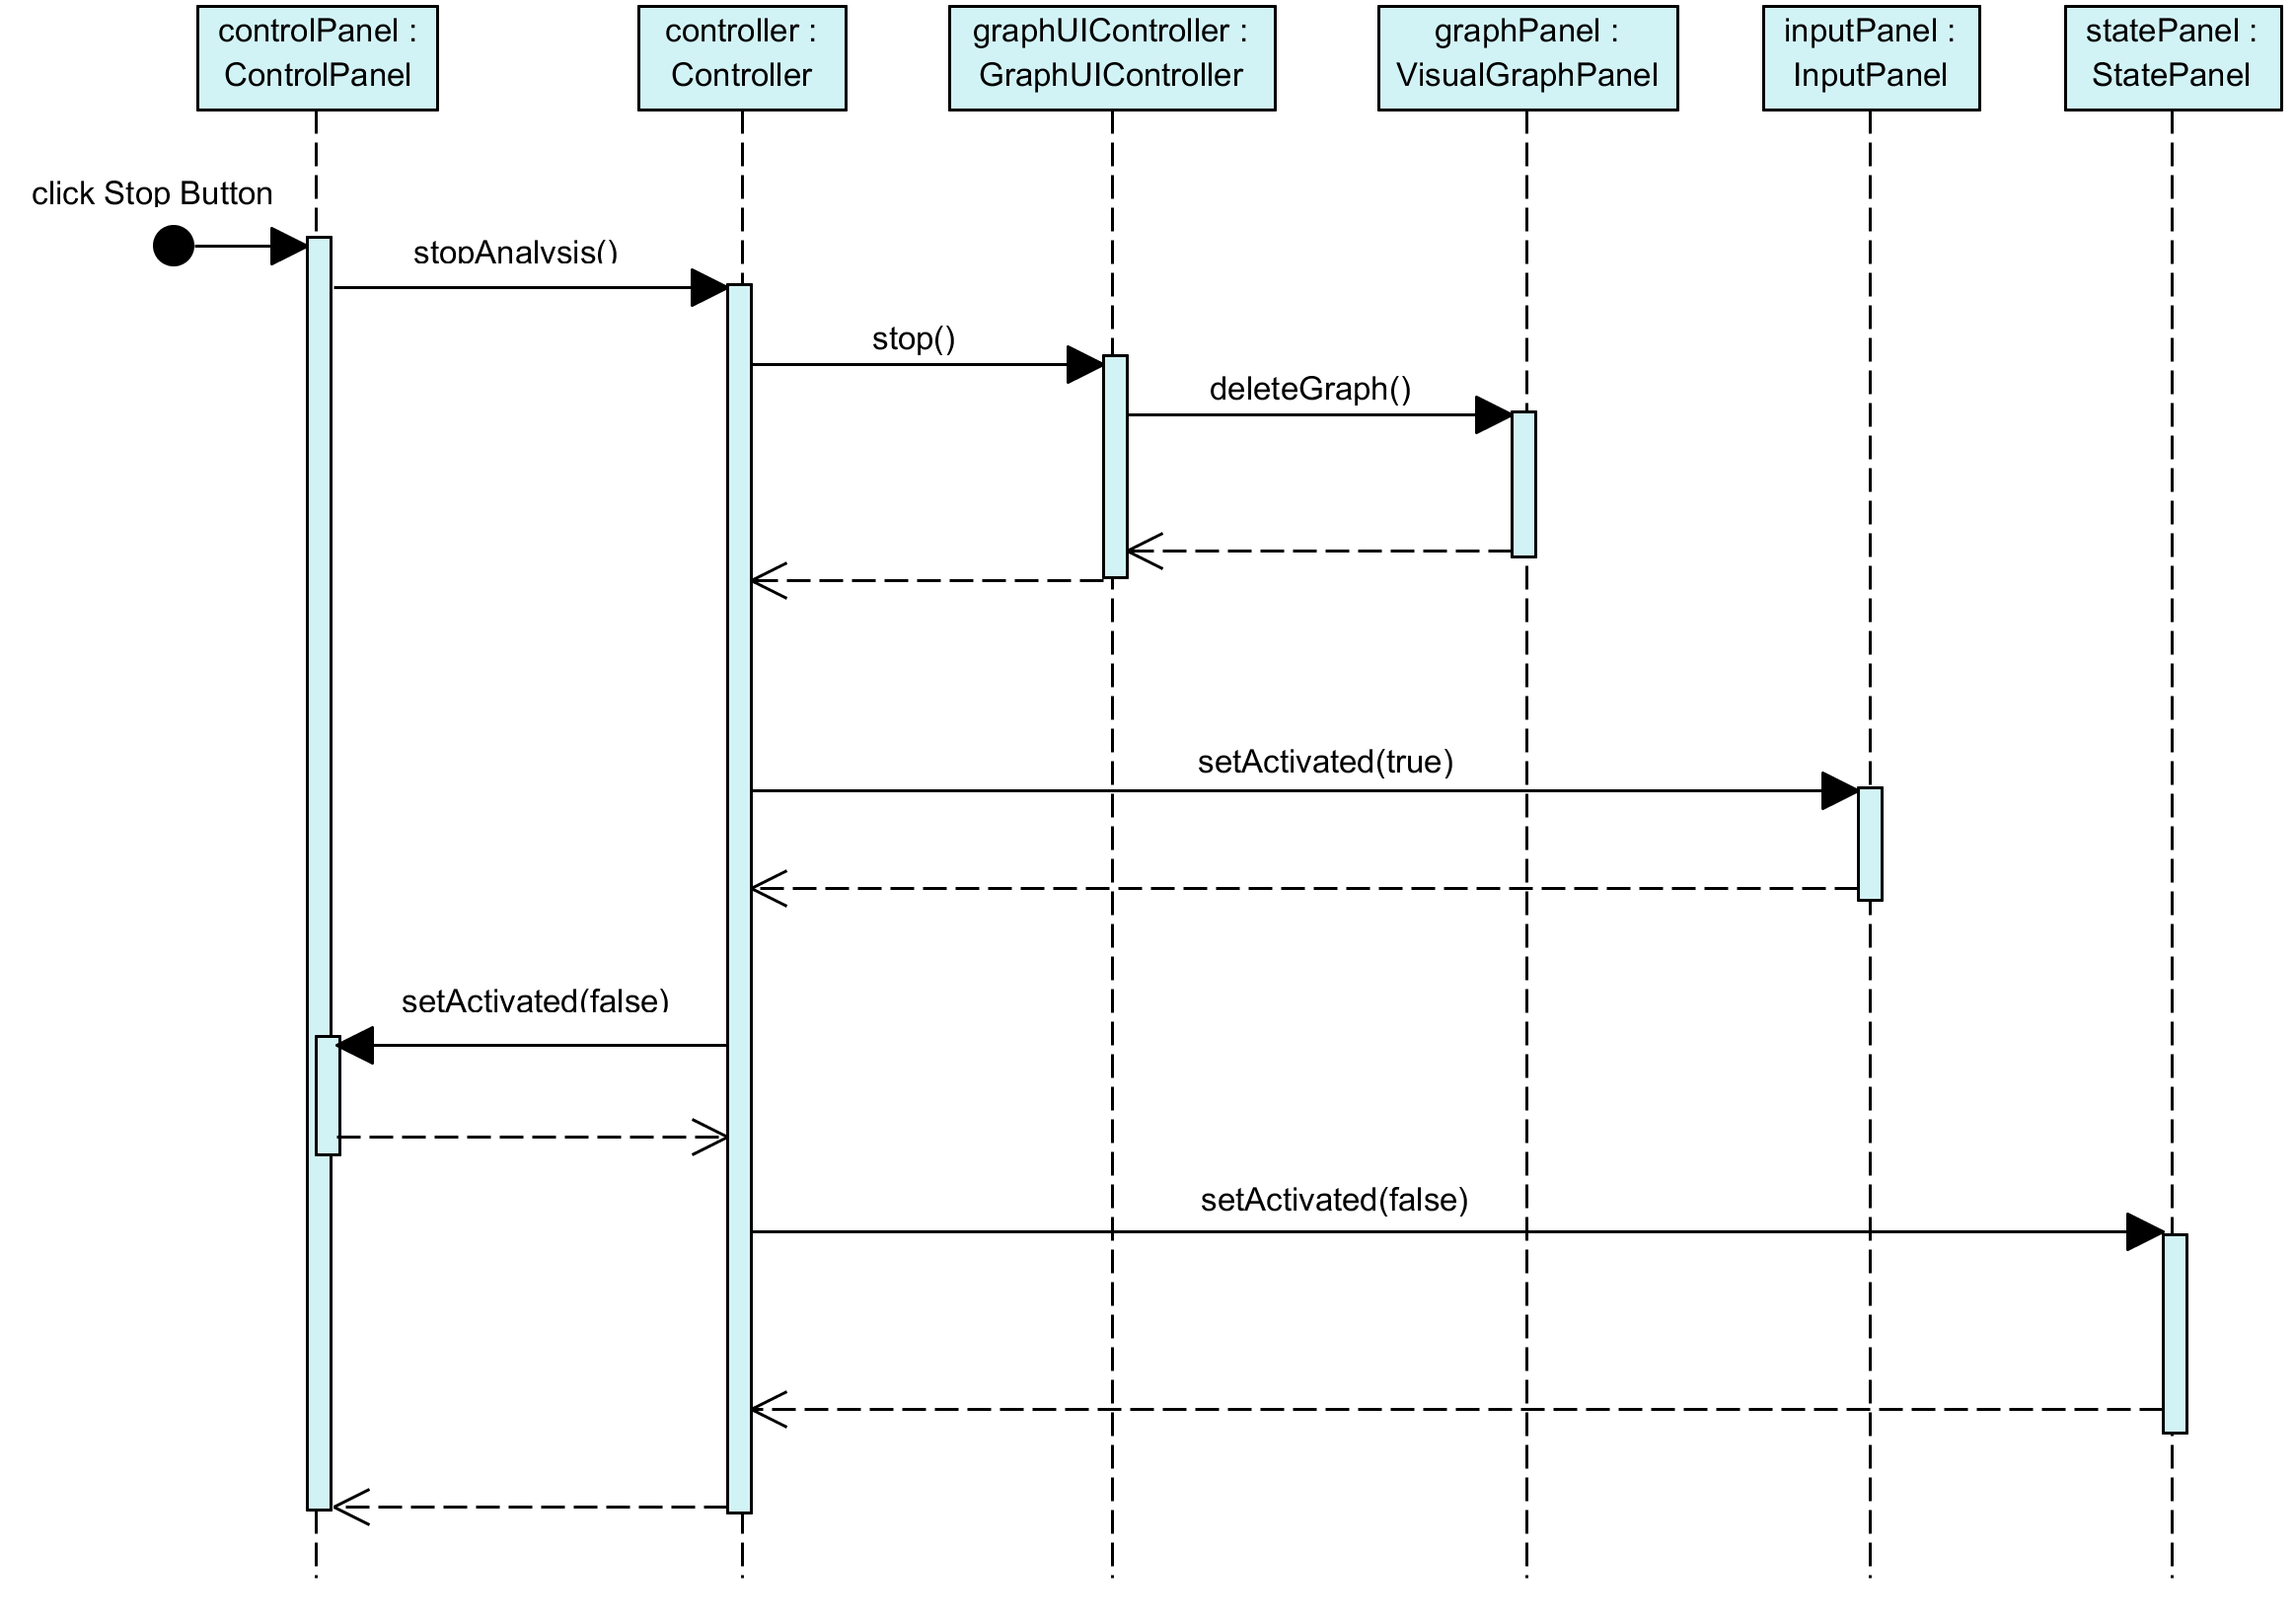
\includegraphics[width=1\textwidth]{Sequenzdiagramme/AnalysisStop}
  \caption{Stoppen der Analyse}
  \label{fig:anaStop}
\end{figure}
\newpage

\section*{Den folgenden Block analysieren}
\begin{figure}[H]
  \centering
    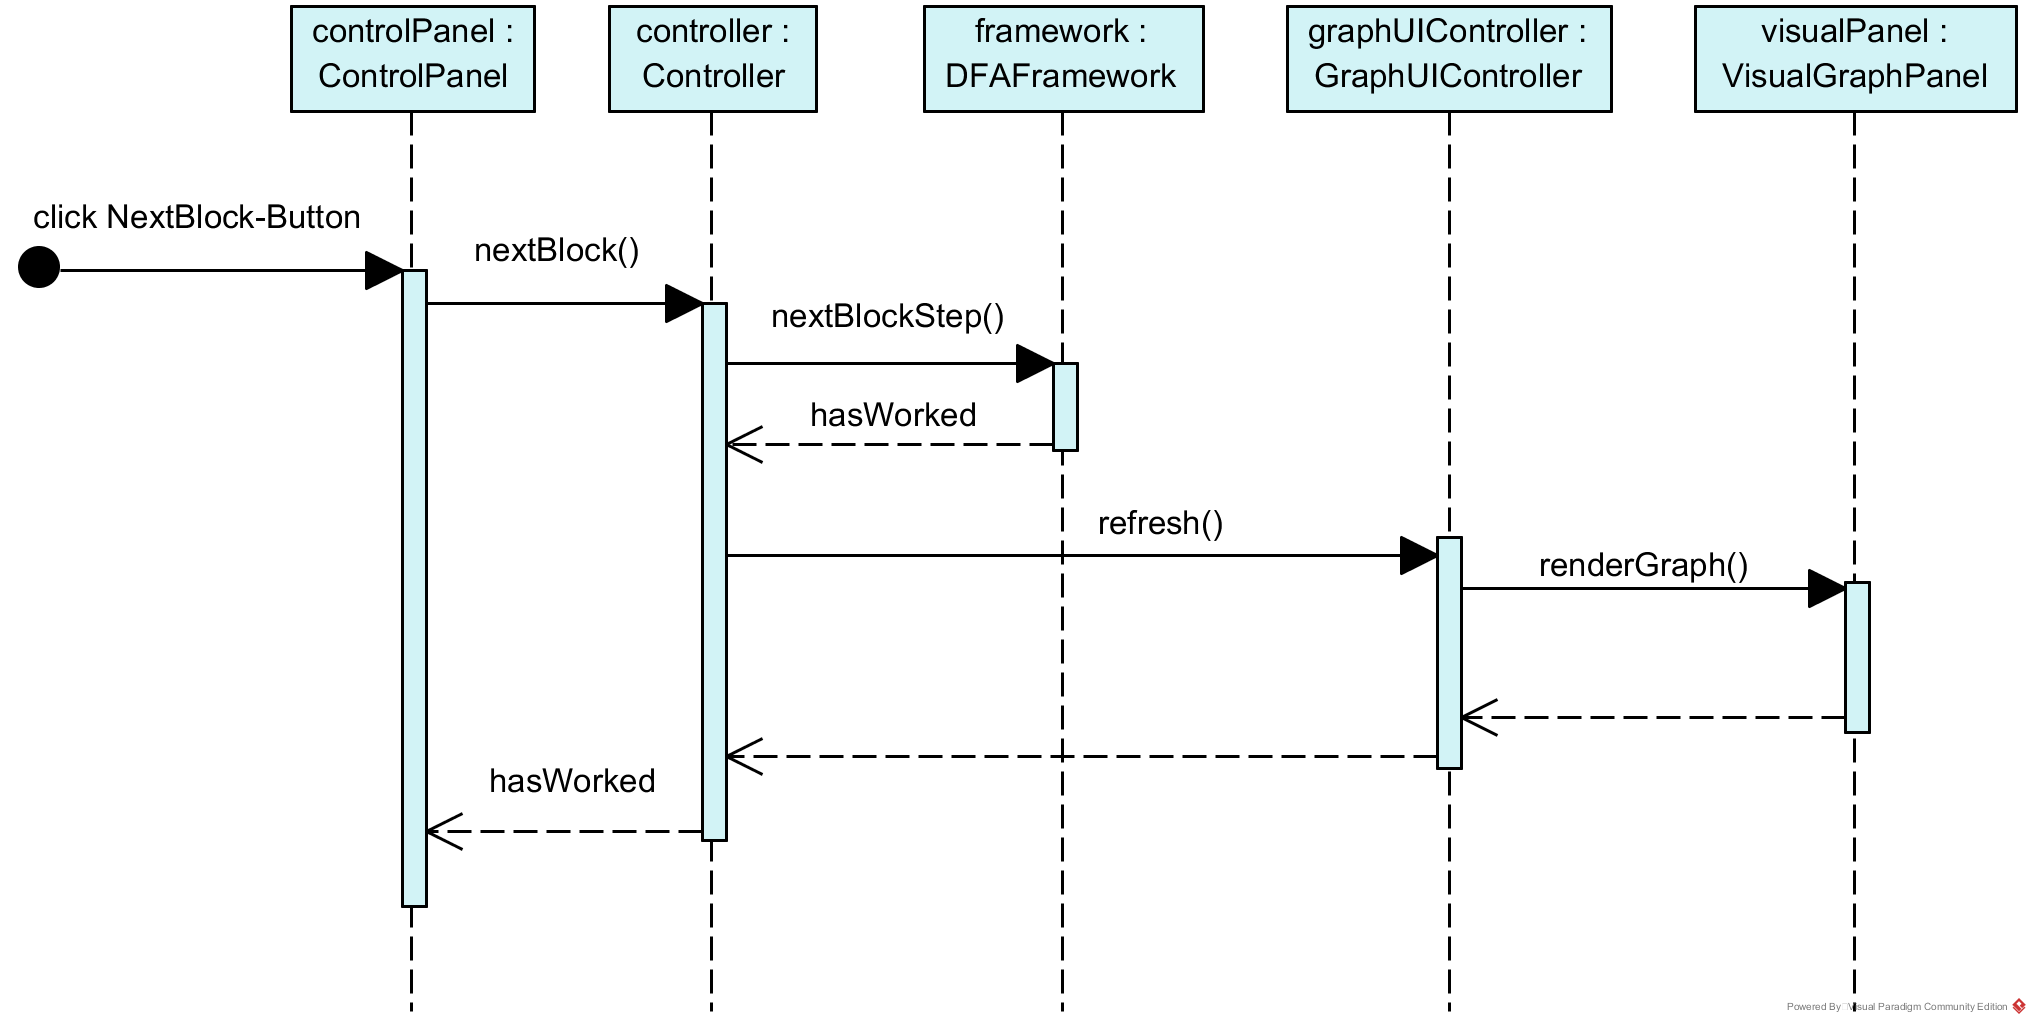
\includegraphics[width=1\textwidth]{Sequenzdiagramme/NextBlock}
  \caption{Den folgenden Block analysieren}
  \label{fig:nextblock}
\end{figure}
\newpage

\section*{Breakpoint setzen}
\begin{figure}[H]
  \centering
    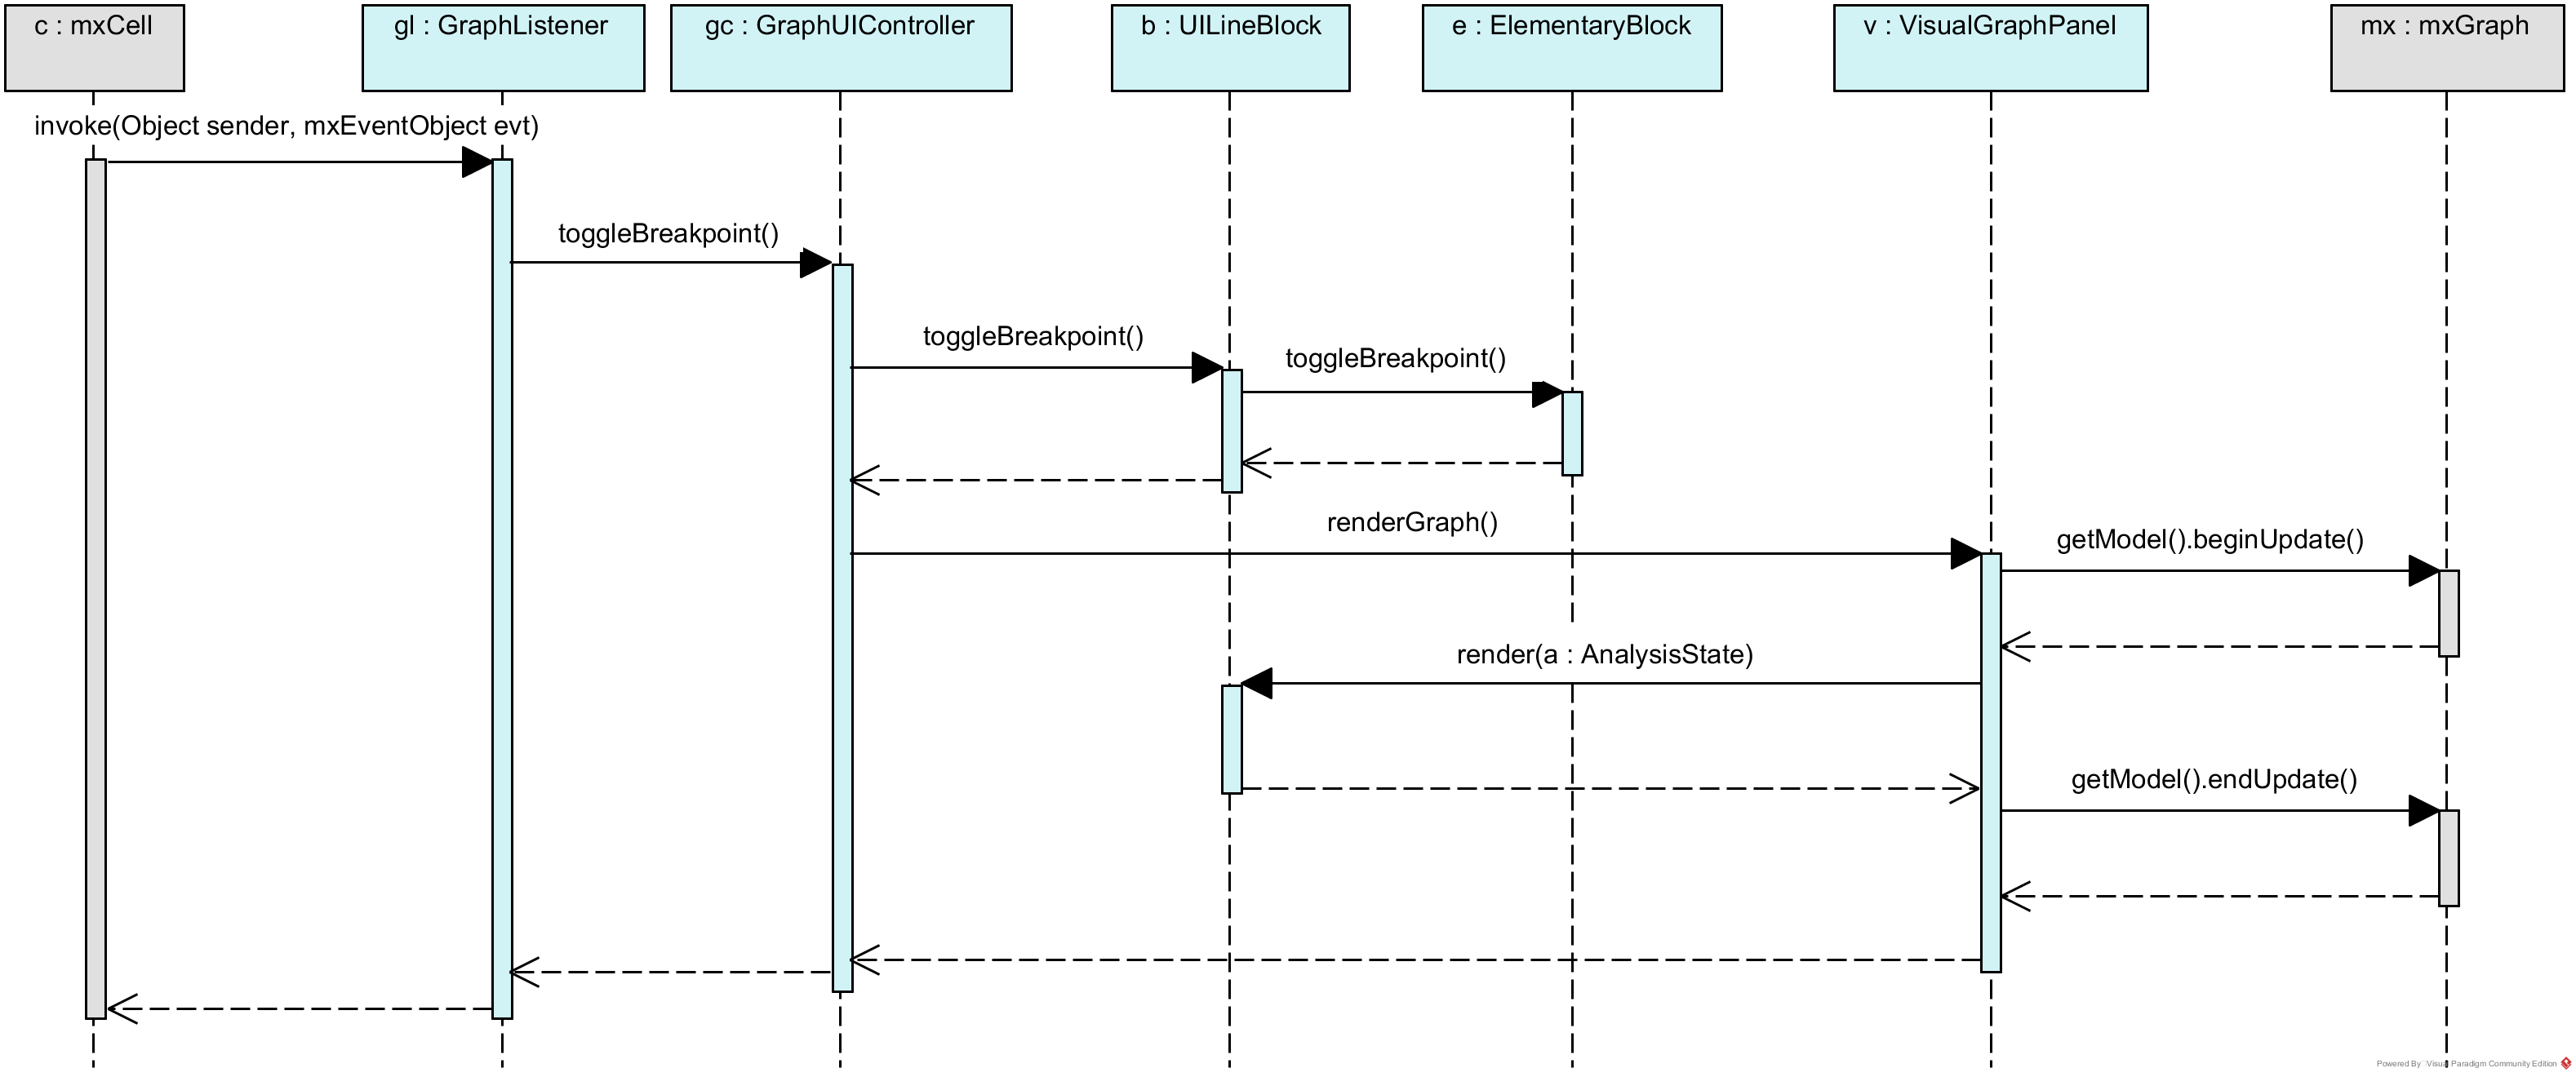
\includegraphics[width=1\textwidth]{Sequenzdiagramme/SetBreakpoint}
  \caption{Breakpoint setzen}
  \label{fig:breakpoint}
\end{figure}
\newpage


\section*{Graphexport}
\begin{figure}[H]
	\centering
	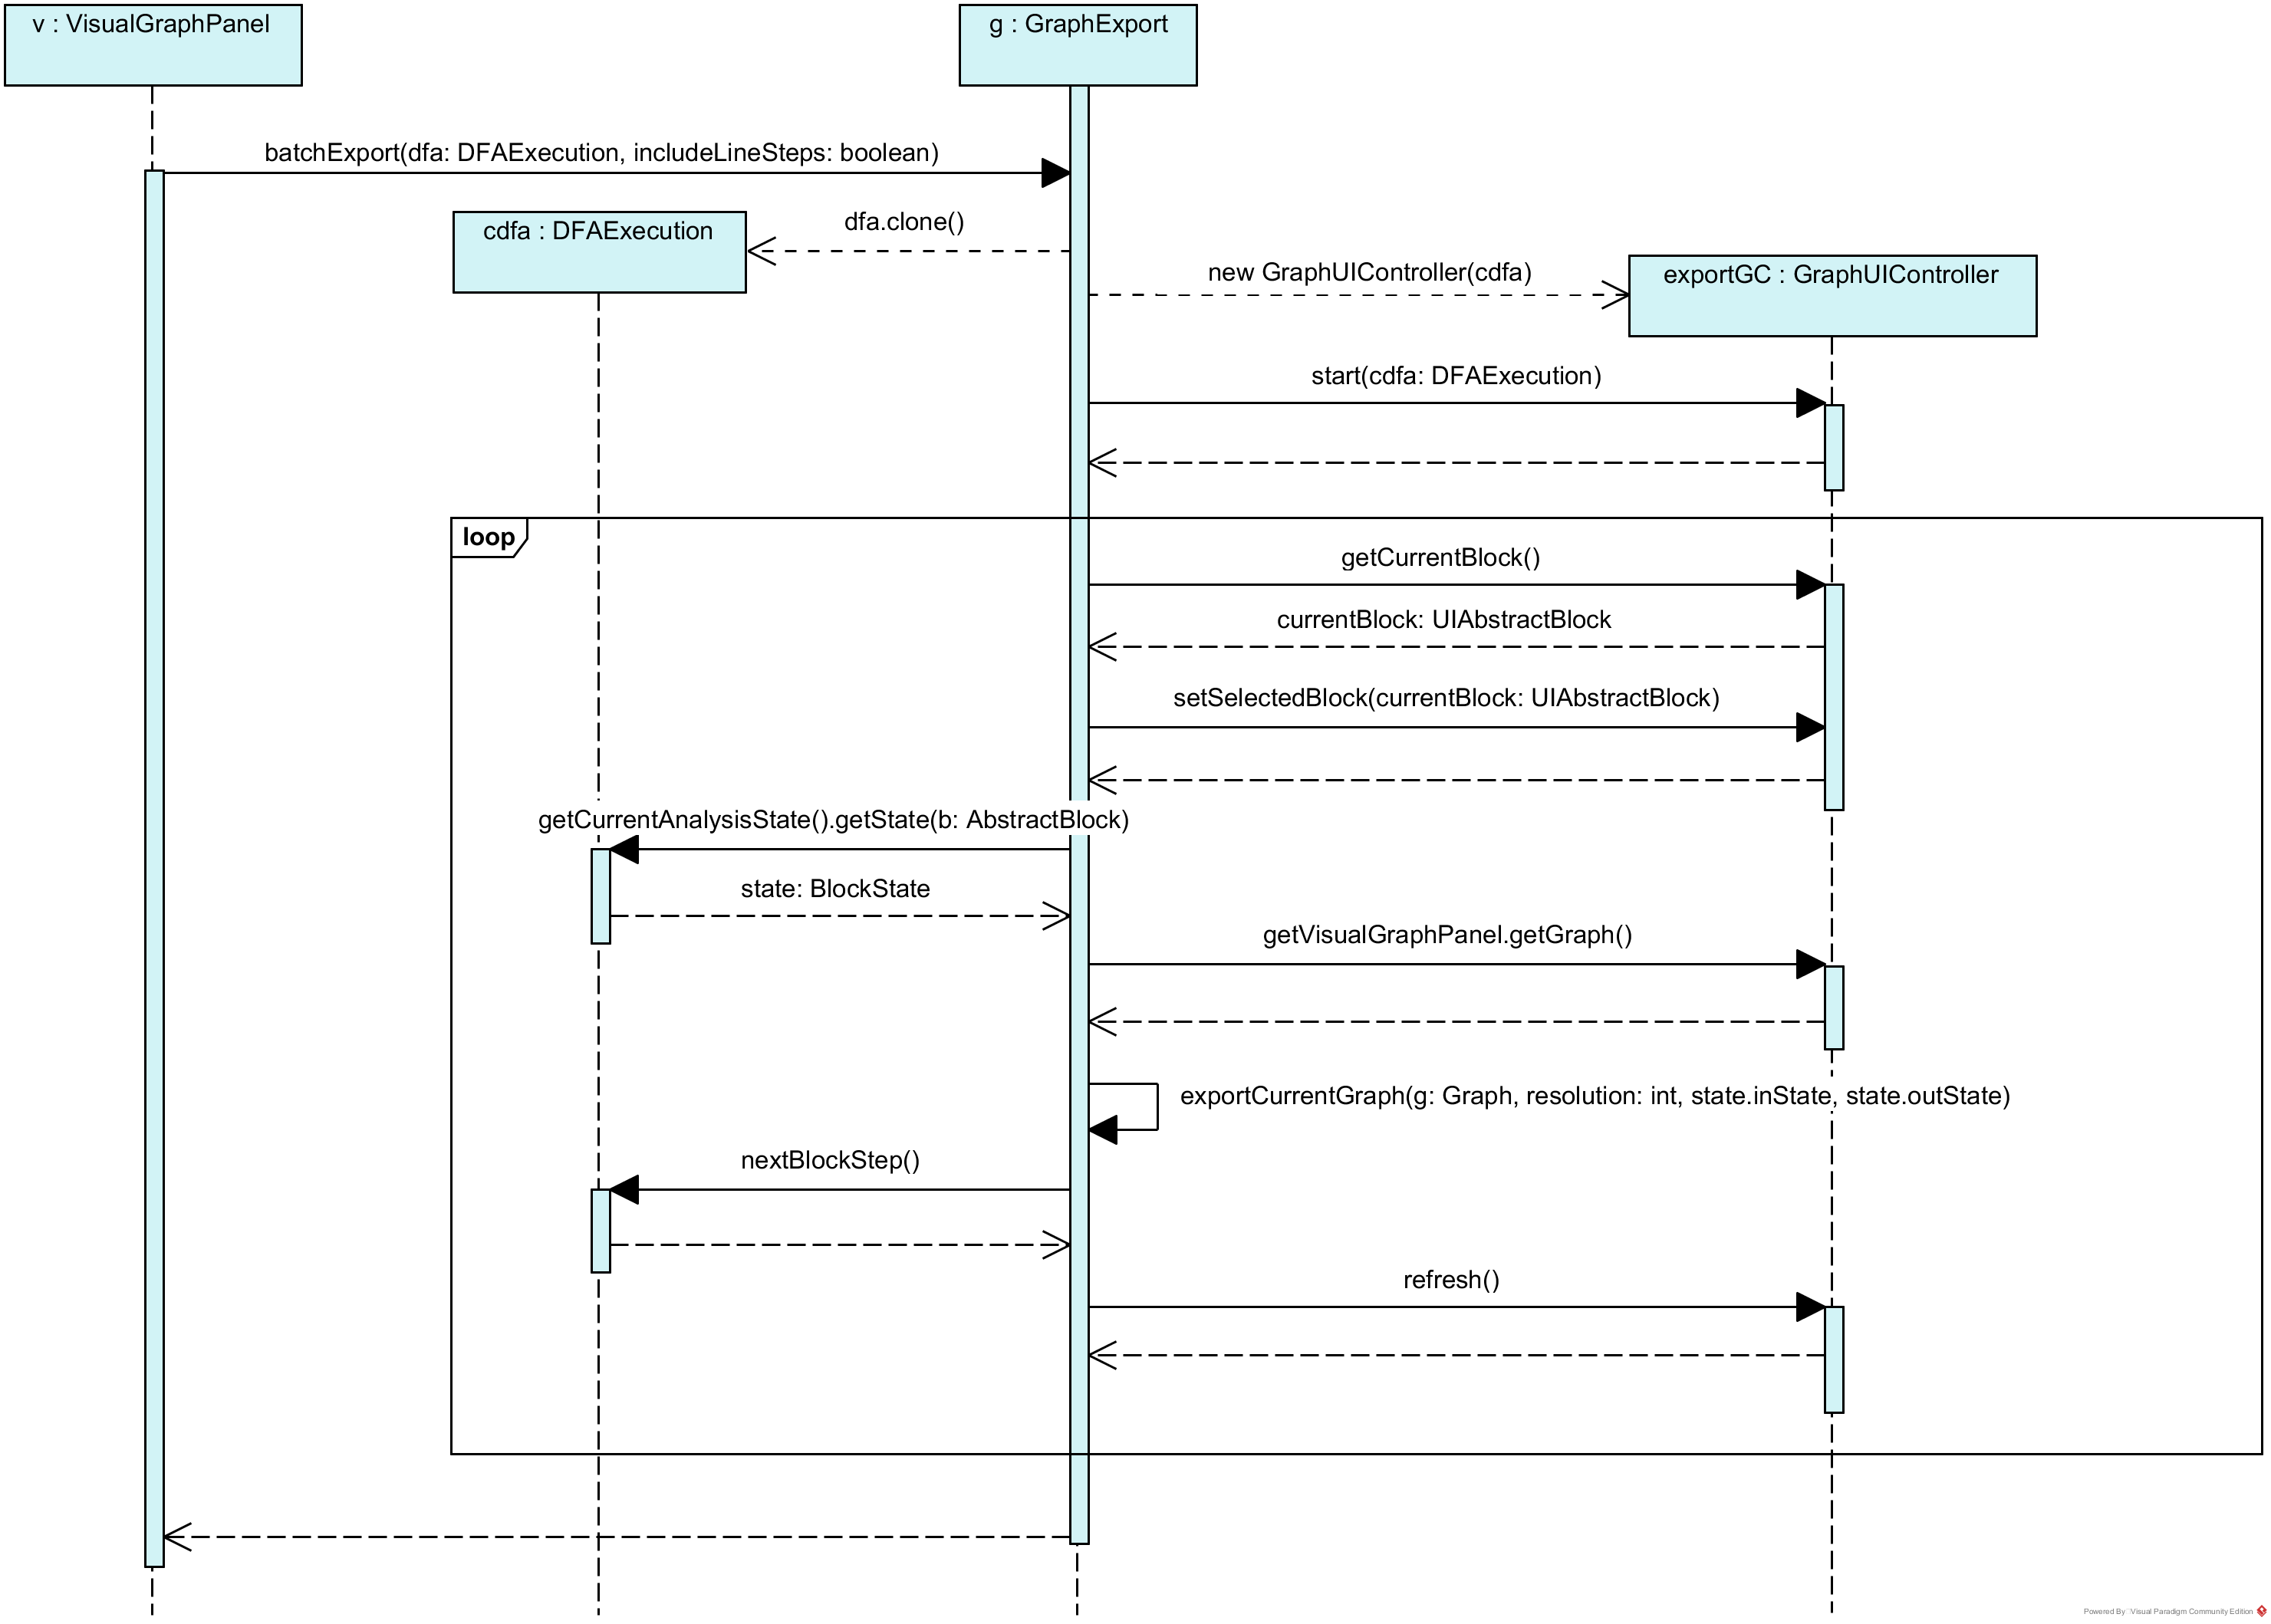
\includegraphics[width=1\textwidth]{Sequenzdiagramme/GraphExport}
	\caption{Export des Graphen}
	\label{fig:graphexport}
\end{figure}
\newpage
